%
% File: chap03.tex
% Author: Your name
% Description: Results 
%
\let\textcircled=\pgftextcircled
\chapter{Methodology}
\label{chap:example}


%%%%%%%%%%%%%%%%%%%%%%%%%%%%%%%%%%%%%%%%%%%%%%%%%%%%%%%%%%%%%%%%%%%%%%
\section{BEEPS Dataset}
\initial{T}he EBRD-World Bank Business Environment and Enterprise Performance Survey (BEEPS) is a joint initiative of the European Bank for Reconstruction and Development (EBRD) and the World Bank. Since the first round in 1999, the BEEPS for Albania has been carried out in 2002, 2005, 2007, 2009, 2013 and 2019. The survey is based on face-to-face interviews with firm (top) managers and owners, conducted by private contractors on behalf of the World Bank, and is designed to yield comparative measurements on many aspects of the business environment. These aspects include general characteristics of the firm, infrastructure and services, sales and supplies, management practices, degree of competition, innovation, capacity, time use of top manager, land and permits, crime, finance, business-government relations, labor, business environment, performance and lastly, environmental policy, regulation and impact. Hence, the BEEPS data-set contains valuable variables to test our hypothesis. The whole population is the non-agricultural economy. Furthermore, the samples of the questionnaire are selected using stratified random sampling. A stratified random sample is one obtained by separating the population units into homogeneous groups, called strata, and then selecting a simple random sample from each stratum. \citep[p. 353]{wooldridge} Thereby, firm size, business sector, and geographic region within a country were used as separation criteria. This methodology stayed the same in all rounds.\footnote{For more detailed information visit the sampling notes on the following website: https://www.enterprisesurveys.org/en/methodology}

It is important to mention that the survey design has been constantly adjusted. This is due to the fact that the biggest disadvantage of BEEPS is missing data, especially for 'sensitive' questions related to corruption. Although this issue has been recognized by the World Bank by adjusting the specific formulations of survey questions and the timing of such questions, plus the fact that the firm's anonymity is maintained, firms respond hesitantly, or not at all. This makes it especially difficult to construct panel models.\footnote{We have investigated the data and unfortunately it was not possible to gain valuable econometric models. The reason for this lies in the fact that (1) variable measurement have changed over time, (2) missing values are a serious issue, and (3) a small sample size.} 
In this regard the following section describes the variables used to test our hypotheses.

%%%%%%%%%%%%%%%%%%%%%%%%%%%%%%%%%%%%%%%%%%%%%%%%%%%%%%%%%%%%%%%%%%%%%%
\section{Variables}
%%%%%%%%%%%%%%%%%%%%%%%%%%%%%%%%%%%%%%%%%%%%%%%%%%%%%%%%%%%%%%%%%%%%%%
\subsection{Explanatory Variables}
We have derived three variables from BEEPS that proxy administrative corruption. The first one, \textit{bribes}, is a numeric variable defined as the percentage of total annual firm sales paid as graft to public officials to 'get things done'. Second, a bribe index is constructed out of six bribe dummy measures related to specific public transactions. Due to high under-reporting we measure the bribe index as a dummy variable equal to one if at least one of the six bribe dummy measures equals one, and zero otherwise. The third measure is tax inspection bribe, which is also a graft measure of a specific public transaction. We use this variable separately because the survey question had comparably high response rates, which would consequently bias the bribe index. This dummy variable may yield specific insights into the relationship of bribes related to tax inspection and firm performance. 
To measure the institutional complexity we constructed a variable named policy obstacle. 
%\renewcommand{\arraystretch}{1.5}
\begin{table}[!h] \centering 
  \caption{Explanatory Variable Description} 
  \label{}
  \begin{adjustbox}{width=\columnwidth,center}
\begin{tabular}{@{\extracolsep{5pt}}lcp{10cm}p{3cm}} 
\\[-1.8ex]\hline 
\hline \\[-1.8ex] 
Variable name & \multicolumn{1}{c}{Binary} & Description & Survey question \\ 
\hline \\[-1.8ex] 
Bribes & No & Percentage of total annual sales paid as informal payment (or in gifts) to public officials to 'get things done' with regard to customs, taxes, licenses, regulations, services etc. & j7a  \\ 
Inspection.Bribe & Yes & A dummy equal to one if a gift or informal payment was expected or requested in a inspection or meeting by tax officials and zero otherwise. & j5 \\ 
BribeIndex & Yes & A dummy equal to one if at least in one of the following public transactions an informal gift or payment was expected or requested: electrical connection, water connection, export customs, import customs, construction-related permit, operating license. & c5, c14, d15a, d5a, g4, j15 \\ 
PolicyObstacle & No & Average score of degree of obstacle (0=no obstacle, 4=very severe obstacle) in the following bureaucratic areas: tax administration, customs and trade regulation, business licensing and permits, and labor regulations. & j30b, d30b, j30c, l30a \\ 
InformalCompetition & Yes & A dummy equal to one if the firm competes against unregistered or informal establishments. & e11  \\ 
\hline \\[-1.8ex] 
\end{tabular} 
\end{adjustbox}
\end{table}

This variable uses the average score of degree of obstacle in four administrative areas: tax administration, customs and trade regulation, business licensing and permits, and labor regulations. The underlying variables are of categorical nature with zero defined as no obstacle, one defined as minor obstacle, two defined as moderate obstacle, three defined as major obstacle and four defined as very severe obstacle. 
Lastly, the informal sector is proxied as a dummy variable if the firm states that it competes against unregistered or informal enterprises. 


%%%%%%%%%%%%%%%%%%%%%%%%%%%%%%%%%%%%%%%%%%%%%%%%%%%%%%%%%%%%%%%%%%%%%%

%%%%%%%%%%%%%%%%%%%%%%%%%%%%%%%%%%%%%%%%%%%%%%%%%%%%%%%%%%%%%%%%%%%%%%
\subsection{Control Variables}
Firm characteristics may influence firm performance and corruption. Therefore, several control variables are added that could possibly confound the measurement effect of corruption on firm performance. 

First, a \textit{sector} dummy variable controls for the industry fixed effects, i.e. if the firm operates in the manufacturing or services sector.

Second, firm \textit{size} is controlled by three dummy variables, i.e. small firms (1-19 employees) , medium firms (20-99 employees), and large firms (100+ employees). Hereby, we control for the fact that larger firms may be able to realize economies of scale and scope. In our regression models, we will leave the \textit{large} dummy variable out so that the matrix has full rank (i.e. dummy variable trap; no rank deficiency). 

\begin{table}[!hb] 
  \centering 
  \caption{Control Variable Description} 
  \label{} 
  \begin{adjustbox}{width=\columnwidth,center}
\begin{tabular}{@{\extracolsep{5pt}}lcp{10cm}p{2cm}} 
\\[-1.8ex]\hline 
\hline \\[-1.8ex] 
Variable name & \multicolumn{1}{c}{Binary} & Description & Survey question \\ 
\hline \\[-1.8ex]
Sector & Yes & A dummy equal to one if the firm is engaged in the manufacturing sector, and zero if the firm is engaged in the retail or other services sector. & a0 \\ 
Small & Yes & A dummy equal to one if the firm has 1-19 employees and zero otherwise. & a6b  \\ 
Medium & Yes & A dummy equal to one if the firm has 20-99 employees and zero otherwise. & a6b \\ 
Large & Yes & A dummy equal to one if the firm has 100 or more employees and zero otherwise. & a6b  \\ 
lnAge & No & Logarithm of firm age [=ln(2019 - year of establishment)] & b5  \\ 
lnExperience & No & Logarithm of years of experience of top manager in sector & b7   \\ 
Foreign & No & Percentage of firm owned by foreign individuals, companies or organizations. & b2b \\ 
Export & No & Percentage of firms sales related to direct exports. & d3c \\ 
TrainingEmployees & Yes & A dummy equal to one if the firm has formal training programs for its permanent, full-time employees and zero otherwise. & l10 \\ 
R\&D & Yes & A dummy equal to one if, over the last three years, the firm has spend on research and development activities within the establishment. & BMh2  \\ 
QualityCertificate & Yes & A dummy equal to one if the firm has an internationally-recognized quality certification. & b8 \\ 
\hline \\[-1.8ex] 
\end{tabular}
\end{adjustbox}
\end{table} 
Third, we control for the \textit{age} (logarithmic) of the firm. It has been shown that as firms mature their profitability declines. (see e.g. \citet{loderer2010firm}) The reason for using the natural logarithm lies in the fact that it narrows the variable range. \citep[p. 221]{wooldridge}

Fourth, the top managers human capital may be a crucial factor influencing firm performance. Therefore, we measure the logarithm of years of sector-\textit{experience} of the top manager.

Fifth, we control for \textit{foreign ownership} by measuring the percentage of the firm held by foreign individuals, companies or organizations. 

Sixth, access to more markets intuitively suggests higher firm performance. Hence, we control for access to foreign markets by measuring the percentage of firms sales related to \textit{direct exports}. 

Seventh, human capital is an important input for firm performance since a skilled workforce may be more productive. Hence, we control for firms having formal \textit{training programs} for their employees.

Eighth, research and development activities (\textit{R\&D}) may influence firm performance. Studies found that R\&D activities have a positive impact on firm performance. (see e.g. BLABLA) Additionally, our models measuring the impact of corruption on innovation activities include the possession of internationally-recognized quality certificates. Quality certificates signal high product quality, which may lead firms to charge a price premium. These surpluses motivate companies to invest in innovation. \citep[p. 218]{paunov2016corruption}
%%%%%%%%%%%%%%%%%%%%%%%%%%%%%%%%%%%%%%%%%%%%%%%%%%%%%%%%%%%%%%%%%%%%%%


%%%%%%%%%%%%%%%%%%%%%%%%%%%%%%%%%%%%%%%%%%%%%%%%%%%%%%%%%%%%%%%%%%%%%%
\subsection{Independent Variables}
%\renewcommand{\arraystretch}{1.5}
\begin{table}[!h] 
  \centering 
  \caption{Independent Variable Description} 
  \label{} 
  \begin{adjustbox}{width=\columnwidth,center}
  \begin{threeparttable}[b]
\begin{tabular}{@{\extracolsep{5pt}}lcp{10cm}p{2cm}} 
\\[-1.8ex]\hline 
\hline \\[-1.8ex] 
Variable name & \multicolumn{1}{c}{Binary} & Description & Survey question \\ 
\hline \\[-1.8ex] 
SalesGrowth\tnote{a} & No & (Nominal)\tnote{*} \, annual sales growth is measured as a percentage change in sales between the last completed fiscal year and a previous period (t=3). & n3, d2  \\ 
EmploymentGrowth\tnote{b} & No & Annual employment growth is the change in full-time employment reported in the current fiscal year from a previous year (t=3). & l1, l2  \\
LaborProductivityGrowth\tnote{c} & No & Annual labor productivity growth is measured by a percentage change in labor productivity between the last completed fiscal year and a previous period, where labor productivity is sales divided by the number of full-time permanent workers (t=3). & n3, d2, l1, l2  \\
InnovationIndex & Yes & A dummy equal to one if the firm at least has introduced any new or improved product or service during the last three years OR if the firm has introduced any new or improved process, and zero if neither of them was introduced. & h1, h5  \\ 
\hline \\[-1.8ex] 
\end{tabular}
   \begin{tablenotes}
     \item[*] We have not adjusted our measures to inflation, as it has not risen significantly.
     \item[a] Formula $=\frac{1}{t}\cdot(\frac{Sales_{t}-Sales_{t-3}} {{(Sales_{t}+Sales_{t-3})/2}}) $ \\
     \item[b] Formula $=\frac{1}{t}\cdot(\frac{Workers_{t}-Workers_{t-3}} {{(Workers_{t}+Workers_{t-3})/2}}) $ \\
     \item[c] Formula $=\frac{1}{t}\cdot(\frac{\frac{Sales_{t}}{Workers_{t}}-\frac{Sales_{t-3}}{Workers_{t-3}}} {{(\frac{Sales_{t}}{Workers_{t}}+\frac{Sales_{t-3}}{Workers_{t-3}})/2}}) $
   \end{tablenotes}
  \end{threeparttable}
\end{adjustbox}
\end{table}
The BEEPS data-set contains various variables measuring firm performance. First, considering firm growth, we focus on three different measures: (1) \textit{annual sales growth}, (2) \textit{annual employment growth}, and (3) \textit{labor productivity growth}. All of these variables, especially (1) and (2), have been used in previous studies, though the measurement is different from ours. (see e.g. blablabla) Choosing more than one measure provides a robustness check for our models. Second, considering firm innovation activities, we focus on a single measure named \textit{innovation index}, which is constructed by the following two dummy variables: (1) innovation related to a new or improved product or service, and (2) innovation related to a new or improved process. The full description of these four independent variables are presented in \textbf{table 3.3}.\footnote{We investigated two more performance variables, i.e. capacity utilization and labor productivity measured as $\frac{\textit{Sales}-\textit{Cost of Sales}}{\textit{\# of employees}}$. We did not include these measures in this study, due to very high under-reporting.}
%%%%%%%%%%%%%%%%%%%%%%%%%%%%%%%%%%%%%%%%%%%%%%%%%%%%%%%%%%%%%%%%%%%%%%

%%%%%%%%%%%%%%%%%%%%%%%%%%%%%%%%%%%%%%%%%%%%%%%%%%%%%%%%%%%%%%%%%%%%%%
\section{Econometric Models}
%%%%%%%%%%%%%%%%%%%%%%%%%%%%%%%%%%%%%%%%%%%%%%%%%%%%%%%%%%%%%%%%%%%%%%
In order to test our hypothesis we employ two different types of econometric models. The first type is a Multiple Linear Regression Model and the second type is a Logit Model.
We begin with the former. Our baseline model, i.e. our model including all control variables, is as follows:
\reqnomode
\begin{equation}\tag{Baseline}
 \begin{split}\label{eq:1}
Y_{i}=\beta_{0}&+\beta_{1}Small_{i}+\beta_{2}Medium_{i}+\beta_{3}lnAge_{i}+\beta_{4}lnExperience_{i}+\beta_{5}Foreign_{i}+\beta_{6}Export_{i}\\
 &+\beta_{7}TrainingProgram_{i}+\beta_{8}RD_{i}+\varepsilon_{i}\\
 \end{split}
\end{equation}

Since we have three different firm growth measures, $Y_{i}$ represents either sales growth, employment growth, or labor productivity growth. 

We can summarize the set of control variables in $\boldsymbol{X}_{i}$ to create some  tidiness:

\begin{equation*}
 Y_{i}=\beta_{0}+\beta_{X}\boldsymbol{X}_{1i}+\varepsilon_{i}  
\end{equation*}

Adding bribes to our baseline model tests for our first hypothesis (H1). Note that we have three different bribe variables, i.e. bribes, bribe index and inspection bribe. 

\begin{equation}\tag{Eq. 1}
 Y_{i}=\beta_{0}+\beta_{X}\boldsymbol{X}_{1i}+\beta_{9}Bribes_{i}+\varepsilon_{i}  
\end{equation}

Adding policy obstacle to the previous equation tests for hypothesis 2a:

\begin{equation}\tag{Eq. 2a}
 Y_{i}=\beta_{0}+\beta_{X}\boldsymbol{X}_{1i}+\beta_{9}Bribes_{i}+\beta_{10}PolicyObstacle_{i}+\varepsilon_{i}  
\end{equation}

To gauge the modifying effect of the institutional environment on the impact of bribes on firm performance (hypothesis 2b) we include an interaction term between the bribe variable and \textit{policy obstacle}:
\begin{equation}\tag{Eq. 2b}
 Y_{i}=\beta_{0}+\beta_{X}\boldsymbol{X}_{1i}+\beta_{9}Bribes_{i}+\beta_{10}PolicyObstacle_{i}+\beta_{11}Bribes*PolicyObstacle_{i}+\varepsilon_{i}  
\end{equation}

To measure the effect of the informal sector on firm performance we incorporate \textit{informal competition}. Hereby, we test for hypothesis 3a. Note that we are not extending the previous equation but testing this hypothesis separately by adding the variable to equation 3.2:

\begin{equation}\tag{Eq. 3a}
\begin{split}
  Y_{i}=\beta_{0}&+\beta_{X}\boldsymbol{X}_{1i}+\beta_{9}Bribes_{i}+\beta_{10}InformalCompetition_{i}+\varepsilon_{i}   
\end{split}
\end{equation}

And lastly, the same way as two steps before, we add the interaction effect of bribes and informal competition to test for hypothesis 3b:

\begin{equation}\tag{Eq. 3b}
\begin{split}
 Y_{i}=\beta_{0}&+\beta_{X}\boldsymbol{X}_{1i}+\beta_{9}Bribes_{i}+\beta_{10}InformalCompetition_{i} \\
 &+\beta_{11}Bribes*InformalCompetition_{i}+\varepsilon_{i}  
\end{split}
\end{equation}
\newline

The second estimation technique is a binary response model since our fourth dependent variable, innovation index, is binary. 
A binary response model can be mathematically described as follows:

\begin{equation}\tag{BRM}
\begin{split}
 P(y=1|\boldsymbol{x})=G(\beta_{0}+\beta_{1}x_{1}+\dotsc + \beta_{k}x_{k})=G(\beta_{0}+\boldsymbol{x}\boldsymbol{\beta}), \quad \text{where} \; 0<G(z)<1
\end{split}
\end{equation}

Following Wooldridge (2012), we write $\boldsymbol{x}\boldsymbol{\beta}=\beta_{1}x_{1}+\dotsc + \beta_{k}x_{k}.$ We are using a logistic function as a nonlinear function for $G$. Hence, the cumulative distribution function for a standard logistic random variable is $G(z)=\frac{exp(z)}{1+exp(z)}=\Lambda (z)$. (p. 612) 

Replacing the right hand side with our control variables, yields the following baseline model: 

\begin{equation}\tag{Baseline 2}
\begin{split}
\boldsymbol{x}\boldsymbol{\beta}=\beta_{X}\boldsymbol{X}_{2i}+\varepsilon_{i}, \quad \text{where} \; \boldsymbol{X}_{2i}=\boldsymbol{X}_{1i}+\text{QualityCertificate}
\end{split}
\end{equation}

The procedure for testing our hypotheses is the same as for the OLS regression above. The only two differences are the estimation technique and the inclusion of one additional control variable.

Hence, we have four different dependent variables and three different key (corruption) independent variables. Each combination yields six model equations. Therefore, we have in total 12 combinations \`{a} 6 equations yielding 72 models. Figure 3.1 on the next page provides a visualization of our methodology.

\begin{figure}[h]%
    \centering
    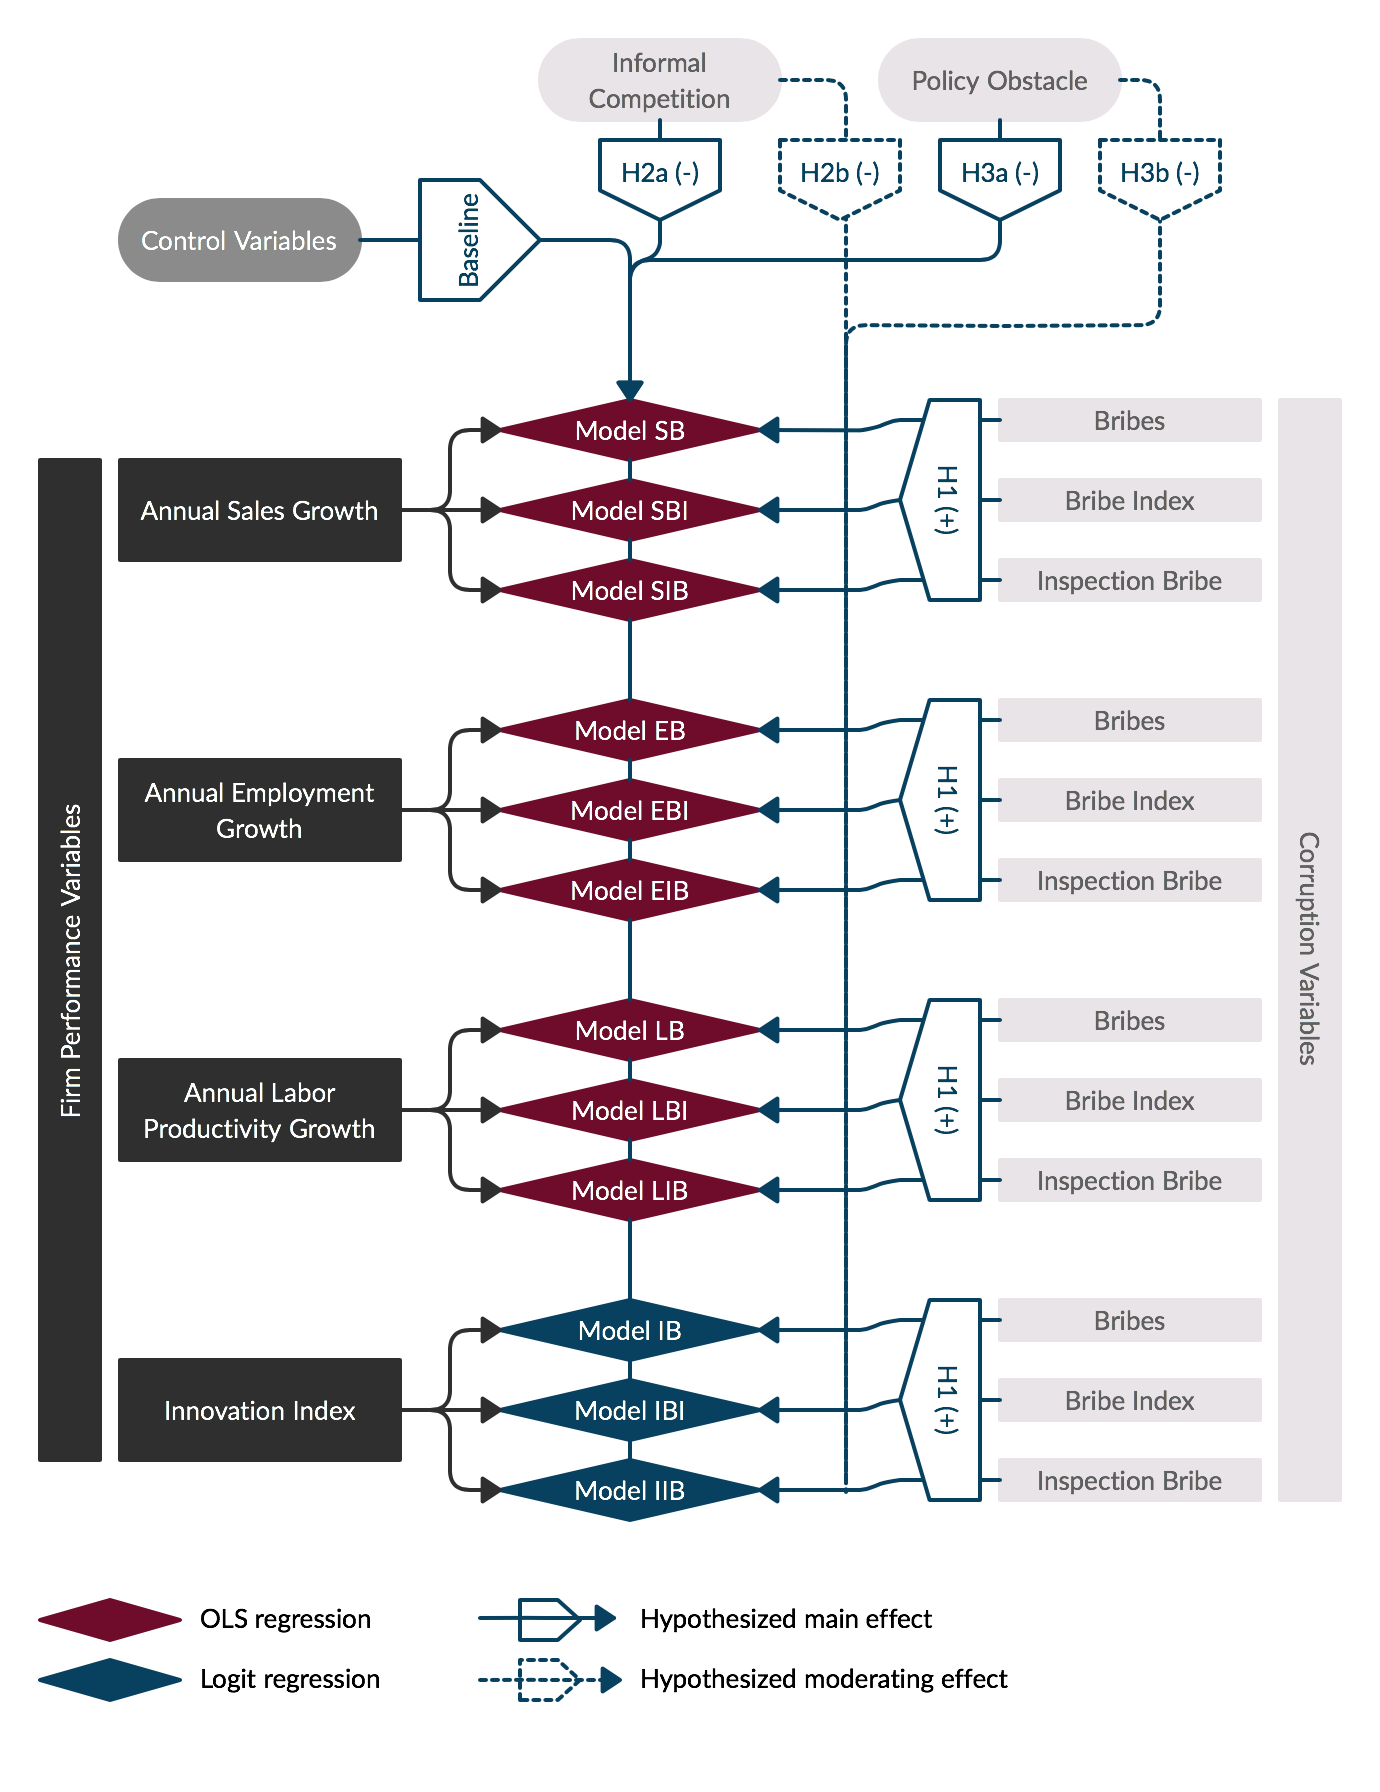
\includegraphics[scale=0.3]{chinchilab-template/Pictures/Flowchart_thesis.png}%
    \caption{Graphical Visualization of Methodology}%
    \label{fig:example}%
\end{figure}